%!TEX root = ../main.tex

\chapter{Introduction}
\label{chp:intro}

\section{Structure of this work}
The following work is structured as described:

\begin{itemize}
    \item \textbf{Chapter \ref{chp:intro}} consists of a general introduction to non-terrestrial networks. Their characteristics are hereby described, and some scenarios are provided where their application would be beneficial. The three main categories of telecommunication satellites are presented, and their characteristics evaluated. Finally, an overview of the possible payload design choices are also presented, as well as a brief description of the potential of multilayered networks.
    \item \textbf{Chapter \ref{chp:ns3}} describes ns-3, the employed network simulator software, highlighting the NTN channel module used as well as its implementation. The reasons behind this choice are hereby detailed.
    Finally, this chapter presents the simulated scenario, describing the characteristics and the parameters of all the involved devices.
    \item \textbf{Chapter \ref{chp:scheduling_problems}} is about the scheduler. The 5G scheduler and its operations in time division duplexing are briefly described, then the main design flaws that arose during the simulations in non-terrestrial scenarios are documented, and the implemented solutions are carefully explained. Some additional observations that were not implemented are hereby described as well, possibly providing some potential starting points for future studies.
    \item \textbf{Chapter \ref{chp:harq}} delves into the problems linked to the operation of the HARQ protocol in a non-terrestrial scenario, discussing the effects of propagation delay as well as the impact of different values of SNR. Some solutions are proposed and evaluated using the ns-3 network simulator.
    \item \textbf{Chapter \ref{chp:conclusions}} finally reports the conclusions of this work, highlighting how the scheduler and HARQ are affected by the characteristics of a non-terrestrial link, summarizing all the solutions that were proposed in this work but still necessitate of a more thorough evaluation, and providing some paths that can be explored in future studies.
\end{itemize}

\section{The non-terrestrial era}
The \ac{3GPP}\footnote{\href{https://www.3gpp.org}{\texttt{3gpp.org}}}, the standardization body tasked with the development of protocols for mobile communication networks, recently put a great emphasis on the importance of the integration of different access technologies along with the existing terrestrial mobile telecommunication infrastructure \cite{3gpp-tr-21.917}.

Specifically, the envisioned future for mobile communications, starting with the already established 5G \ac{NR} and further expanding with the new sixth-generation cellular networks (6G), foresees the integration of a new non-terrestrial component. The latest \ac{3GPP} releases (Rel. 17 and Rel. 18) require 5G and 6G networks to be able to provide non-terrestrial satellite access complementing the already existing terrestrial access technologies \cite{overview-rel-17-18-saad, 5g-nr-communication-geo-leo-maattanen}.

To give a proper definition, the term \ac{NTNs} refers to a category of networks where at least one link is routed via an aerial or space-borne vehicle such as \ac{HAPs}, \ac{UAVs} or telecommunication satellites.

\section{Limitations of terrestrial networks}
In order to explain the motivations behind the choice of expanding the current terrestrial infrastructure, the following sections present a few scenarios where the current terrestrial infrastructure fails to provide an adequate service due to some of their intrinsic limitations, and \ac{NTNs} can help to provide a better coverage.

\begin{figure}[ht]
    \centering
    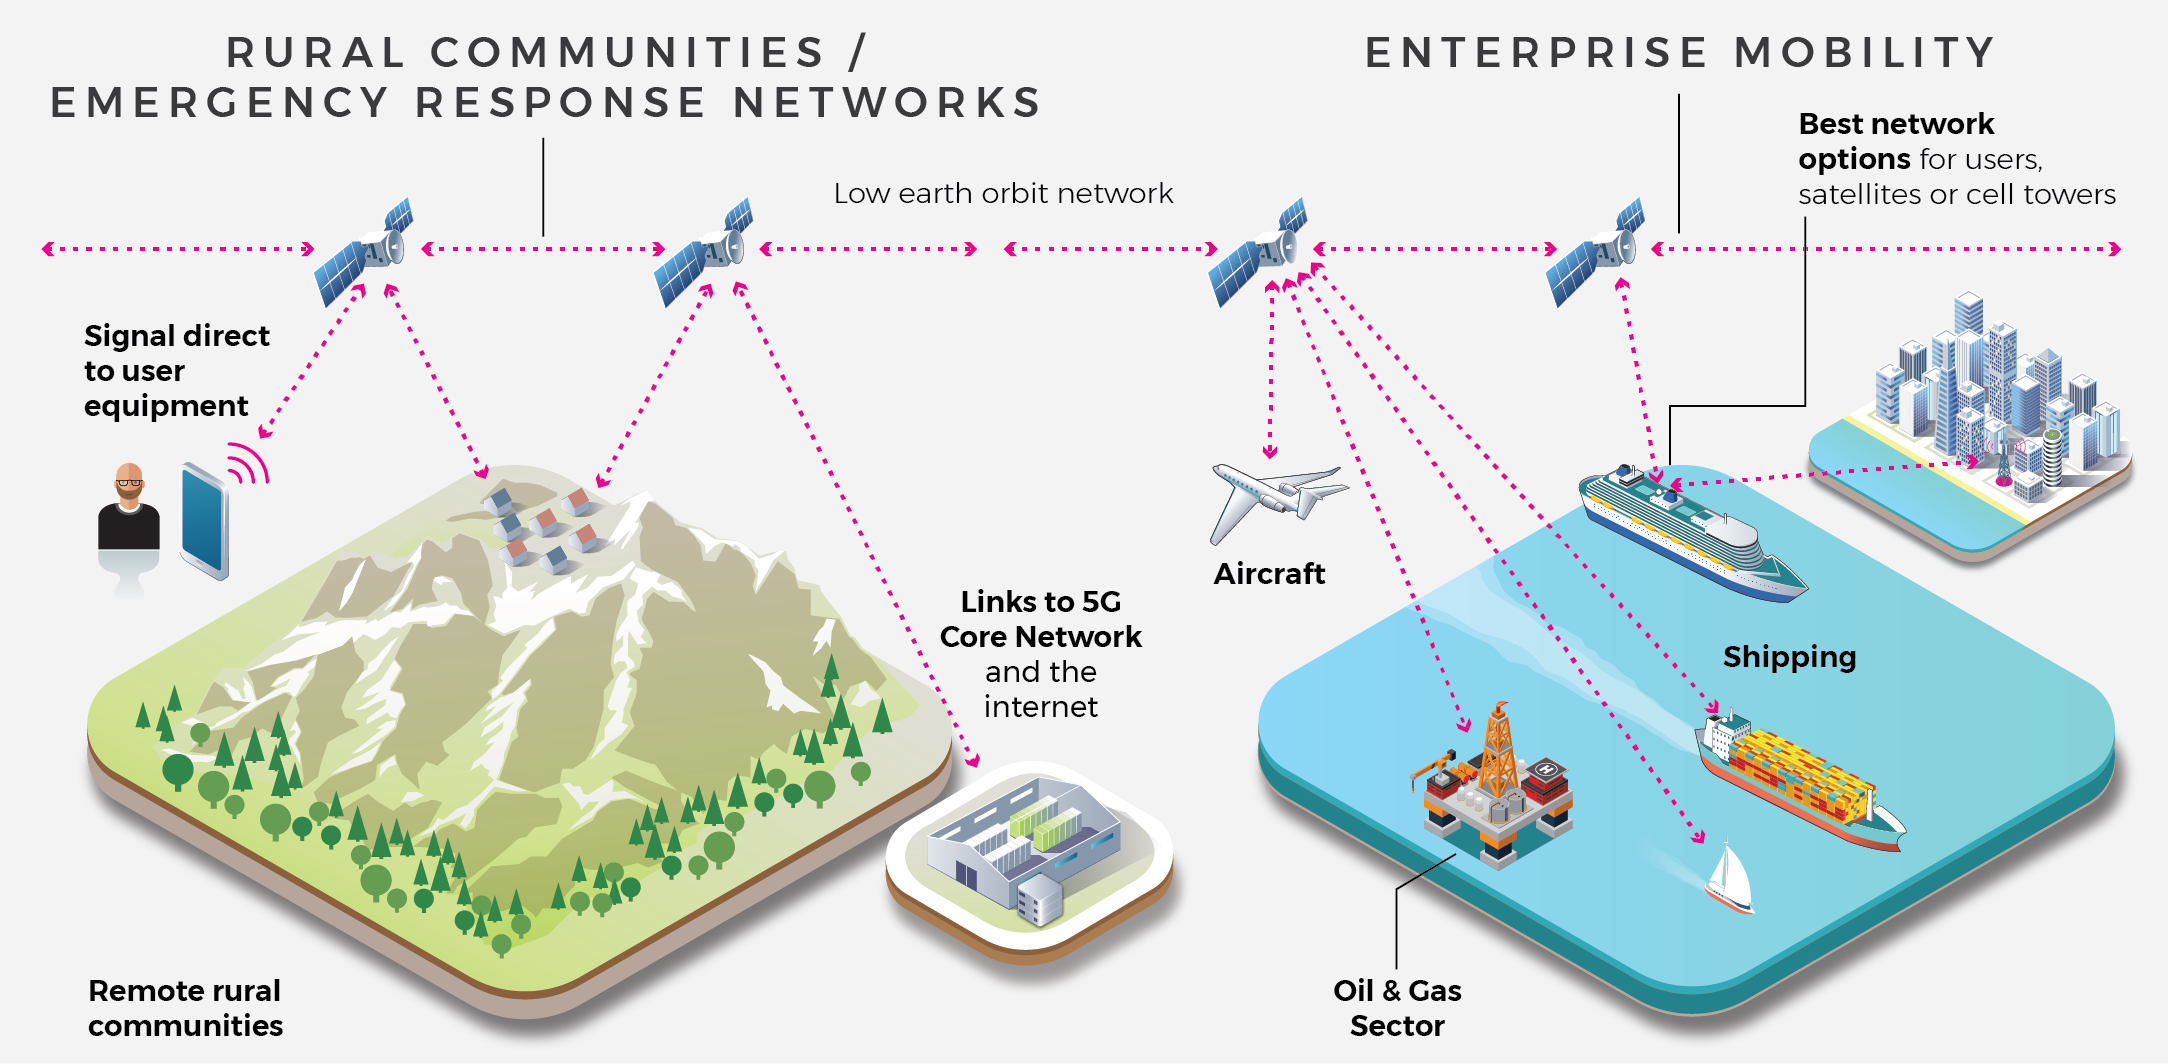
\includegraphics[width=0.9\textwidth]{res/sat-usecases.png}
    \caption{NTN use cases, courtesy of \href{https://telecominfraproject.com/ntcs/}{telecominfraproject.com}}
    \label{fig:sat-use-cases}
\end{figure}

\subsection{Remote places}
While \ac{TN} make the well-established foundation of today’s mobile communication infrastructure, their own nature poses some intrinsic limitations to their deployment in certain scenarios, especially in contexts of rural and remote areas. Conditions such as harsh terrain and geographical impediments like mountain ranges and large bodies of water act as natural barriers to the deployment of terrestrial infrastructure. Moreover, the need for ground equipments such as base stations and networking gear requires the presence of an already established and reliable power grid, further driving up the costs that telecommunication companies would have to sustain to bring connectivity in isolated areas without such amenities.

\paragraph{Population density}
The population density in remote and rural places is typically much lower than the one found in cities, and users are spaced in vast areas of land. Because of this reason, the investment that has to be made on a per-user basis in order to provide coverage would be much higher compared to a more urbanized scenario, where potential users are more densely distributed. The already high infrastructure cost will therefore have a hard time generating any profit, making this kind of market even more unattractive to private investors and further limiting the possibility for the people living there to access the internet, a resource which is becoming increasingly more important as time goes by.

\paragraph{Opportunities}
As studied and documented in \cite{6g-challenge-opportunity-base-pyramid}, the issue of an inadequate broadband coverage in rural regions is an enormous challenge. Providing connectivity to the half of the world population living in rural or underprivileged areas requires a colossal effort, but it would also be a unique opportunity to kick-start the economy of currently underdeveloped countries. Access to the Internet would provide the population a possibility to progress on the educational, environmental, business and health planes, promoting a more fair access to information and alleviating the problem of digital divide between different parts of the world.

\subsection{Redundancy and additional capacity}
Another limitation of the current terrestrial infrastructure is the lack of redundancy and robustness against natural disasters. Extreme events such as earthquakes, hurricanes, fires and floods, but also deliberate behaviors such as targeted attacks by terrorist organizations and sabotages can disrupt the connectivity, leading to outages that can potentially last for a long period of time. This in turn can cause significant economical damage and, in emergency situations, hinder the already difficult rescue efforts, potentially even leading to loss of lives.

The simple installation of additional base stations is not a viable solution because they would all share the same weaknesses, and extreme events such as tornados would easily be able to render all the additional equipment useless. The cost of essentially doubling the existing access network to make it more resilient would be enormous.

In this scenario, \ac{NTNs} can act as a redundant access methodology to decrease the downtimes of terrestrial infrastructure, providing emergency communication services as well as additional capacity when required.

Fig. \ref{fig:multiple-connectivity}, courtesy of \cite{3gpp-tr-38.811}, shows a scenario where terrestrial and non-terrestrial access technologies are used transparently to access the network. It depicts a \ac{UE} that can use both the non-terrestrial link provided by the satellite or the terrestrial one. In this case, the satellite is connected to a ground gateway where the \ac{gNB} is located, therefore only rerouting the signal coming from the \ac{UE}.

\begin{figure}[ht]
    \centering
    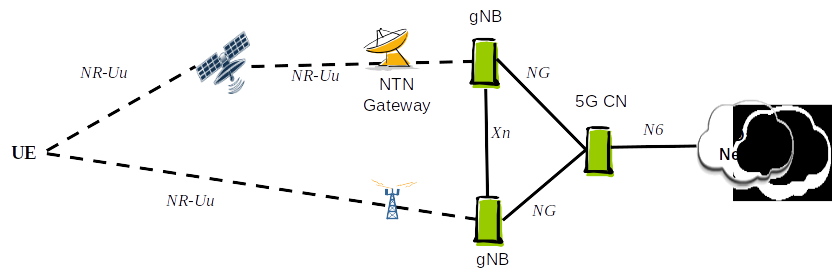
\includegraphics[width=0.7\textwidth]{res/multiple-connectivity.png}
    \caption{Transparent use of multiple radio access technology \cite{3gpp-tr-38.811}}
    \label{fig:multiple-connectivity}
\end{figure}

\subsection{Long distances and sensors}
Remote equipment, offshore plants and distribution grids will also benefit from the research carried out in this field, since providing terrestrial connectivity in those scenarios is a very challenging task due to the physically long distances involved. The installation of an underwater optical fiber link to serve a single endpoint, such as an offshore oil rig or power plant located in the open ocean, would bear a disproportional cost compared to the functions required, and providing maintenance would be another challenging and expensive task. 
The deployment of non-terrestrial networks would be the easiest way to provide connectivity on a global scale, therefore allowing internet access in isolated places without the need for an expensive, dedicated connection.

Consider now the problem of connecting a number of sensors sparsely distributed in a large area. When distances are large, solutions may be either the densification of radio stations or the use of a lower frequency in order to have a less severe propagation loss. However, those approaches have their downsides and are not always feasible, requiring costly, ad-hoc solutions tailored for each specific scenario. In this case, the vast coverage area of \ac{NTNs} will undoubtedly be useful to provide internet connection \cite{performance-ntn-support-iot-wang}.

\paragraph{} Other scenarios where \ac{NTNs} can become useful in overcoming the limitation of their terrestrial counterpart are well described in \cite{ntn-6g-era-challenges-giordani} and \cite{potential-multilayered-nierarchical-ntn-wang}.

\section{Satellite types}
\label{sec:satellite-types}
Satellites are divided in three main different categories depending on their orbiting altitude: \ac{GEO}, \ac{MEO}, and \ac{LEO} satellites. Each one has its own characteristics, presenting some upsides and downsides as described below. Fig. \ref{fig:satellite_coverages} illustrates the different orbiting altitudes as well as an approximate idea of the different coverage areas for each orbit.

\begin{figure}[ht]
    \centering
    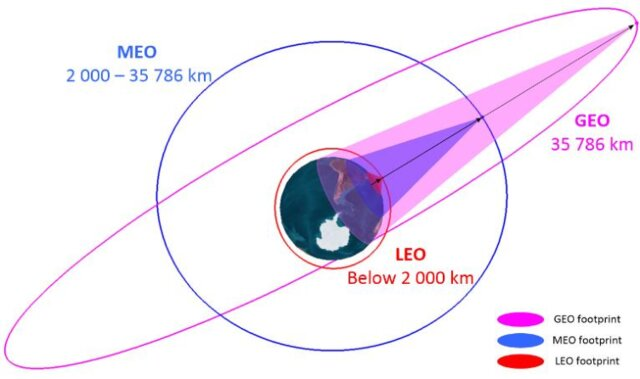
\includegraphics[width=0.9\textwidth]{res/satellite-coverages.jpg}
    \caption{Height and approximate coverage areas for satellites at different orbits \cite{sustainable-sat-com-6g}}
    \label{fig:satellite_coverages}
\end{figure}

\subsection{GEO satellites}
Orbiting at a height of 35.786Km, to an observer placed on the Earth surface \ac{GEO} satellites appear stationary, since their orbiting period is the same as the Earth rotational period.

\paragraph{Advantages}    
Since \ac{GEO} satellites are geostationary, continuous coverage to a designated area can be provided using as little as a single satellite, while the use of non-\ac{GEO} satellites would require the deployment of a constellation, which is both more complex and more expensive. 

This also vastly simplifies the problem of the ground equipment having to be able to track the satellite. Since the satellite position is always known, once the position of the \ac{UE} is established, the relative position of the satellite can be easily calculated.

As shown in Fig. \ref{fig:satellite_coverages}, the high altitude of \ac{GEO} satellites creates a large cell footprint. While the deployment cost of a single \ac{GEO} satellite is higher than both \ac{MEO} and \ac{LEO} ones, the cost per coverage area is overall lower, and an almost full coverage of the terrestrial globe can be achieved using only three equally spaced satellites \cite{types-of-orbits-esa}.

\paragraph{Disadvantages}
The disadvantages of \ac{GEO} satellites are mainly linked to the large distance with \ac{UE}s places on the Earth surface: the transmission power and the antenna gain have to be high enough to overcome the greater propagation losses, and the propagation delay of the signal adds about 120ms to the overall latency. This means that if the \ac{UE} sends a request to a server at $t=0$ through a \ac{GEO} link, the packet will be received by the destination node at least at $t=240$ms. The response will then finally reach the \ac{UE} after at least $480$ms from the initial transmission, and these calculations do not factor in any delay related to medium access requests, packet transmission times and processing delays, which would further increased the overall latency.

In addition to the positive aspects previously discussed, the large cell footprint also brings some downsides with it. Due to the vast area, a single satellite will be required to serve a massive number of users, so the total available capacity will have to be shared between a bigger number of equipments, and the throughput experienced by each of them will be reduced.

Solutions to provide a greater capacity have been proposed and are currently in the early stage of studies, such as the use of beamforming to divide the covered area in smaller cells and the employment of higher frequency bands towards Ku, K and Ka as depicted in Fig. \ref{fig:satellite-bands} \cite{advances-comm-sat-sys}.
Moreover, the high number of users also leads to a large rate of initial access requests, with the possibility of channel saturation as described in \cite{3gpp-tr-38.811}.

\begin{figure}[ht]
    \centering
    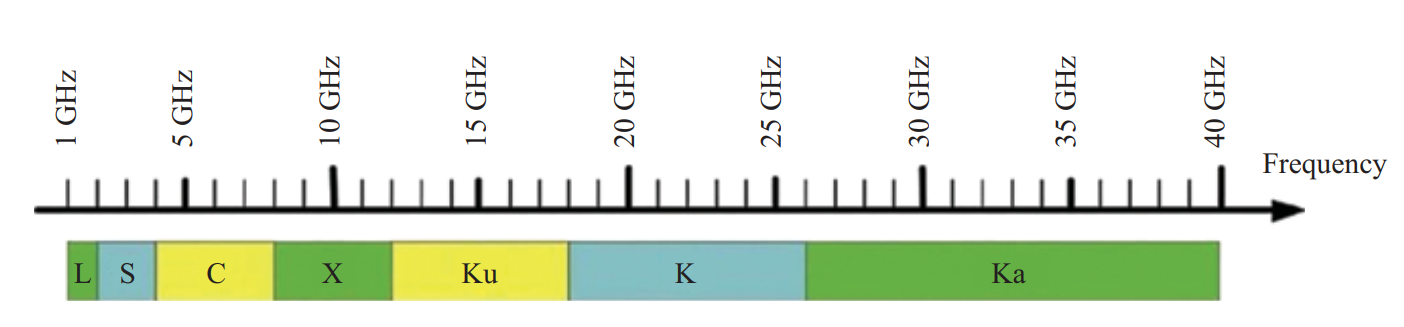
\includegraphics[width=0.9\textwidth]{res/satellite-bands.png}
    \caption{Satellite spectrum bands allocation \cite{advances-comm-sat-sys}}
    \label{fig:satellite-bands}
\end{figure}

\subsection{MEO satellites}
\ac{MEO} orbit is comprised between \ac{LEO} and \ac{GEO}, therefore all satellites orbiting between 2000Km and 35.786Km are considered as \ac{MEO}. This vast orbital space is mainly used by navigation systems such as GALILEO \cite{types-of-orbits-esa}.

The propagation delay can vary a lot depending on the altitude, but it is larger than \ac{LEO} and smaller than \ac{GEO}. The same point can be made regarding the cell size and number of served users. 

As for \ac{LEO} satellites, \ac{MEO} ones do require a constellation in order to provide continuous coverage over a designated area, since they are not geostationary. The numerology of the constellation, however, is smaller than the one required for \ac{LEO} satellites, since each platform can serve a larger area.

Their peculiarity of presenting many of the downsides that characterize both \ac{GEO} and \ac{LEO} satellites, while being unable to offer any substantial benefit over their competitors besides the need for a smaller constellation, makes them less than ideal candidates for applications in non-terrestrial networks.

\subsection{LEO satellites}
\label{sec:leo}
Orbiting below the threshold altitude of 2.000Km, \ac{LEO} satellites are the most promising solution in the realm of \ac{NTNs} mainly because they can offer really advantageous throughput and propagation delay. The disadvantages and complications are however many, but their benefits overshadow them.

\paragraph{Advantages}
The lower altitude entails a shorter propagation delay, on the order of about 6ms, and the smaller coverage area of each satellite depicted in Fig. \ref{fig:satellite_coverages} means that the total number of users that need to be served is smaller. This also allows the use of higher frequency bands and the constraints of high antenna gains are less stringent compared to \ac{GEO} satellites, since the experienced path loss is much smaller. This in turn enables the achievement of higher overall throughputs, more suited to satisfy the requirements of modern days broadband connectivity, as detailed in \cite{satellite-communication-mmwave-giordani}.

While not being numerous, those advantages are enough to make \ac{LEO} satellites the most promising choice in the field of \ac{NTN}s.

\paragraph{Disadvantages}
The cost per deployed satellite is significantly smaller than \ac{GEO} and \ac{MEO} satellites, and multiple deployments within a single launch are possible, driving the costs further down. However, given that \ac{LEO} satellites are not geostationary, a large constellation is needed to provide a continuous service, driving the deployment costs significantly up. As an example of how vast those constellations can become, Fig. \ref{fig:starlink_constellation} depicts the \ac{LEO} satellites employed by Starlink\footnote{Starlink is a satellite internet constellation operated by Starlink Services, LLC, a wholly-owned subsidiary of American aerospace company SpaceX.}, counting about 4.808 units in service at the time of writing\footnote{Source: \href{https://satellitemap.space/}{\texttt{satellitemap.space}}}.

\begin{figure}[ht]
    \centering
    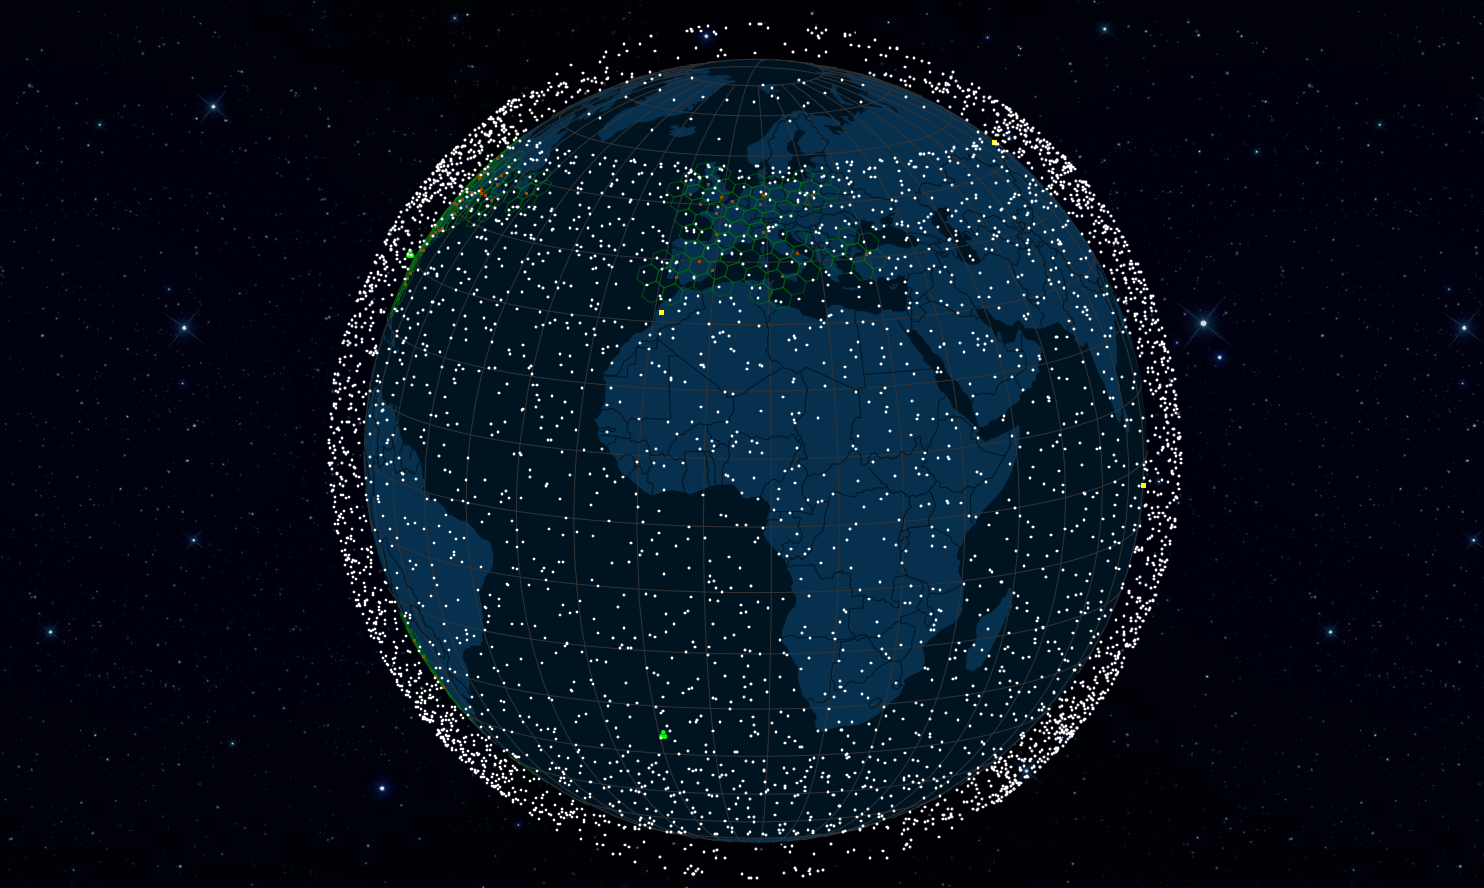
\includegraphics[width=0.9\textwidth]{res/starlink-constellation.png}
    \caption{Starlink constellation as July 2024. Source: \href{https://satellitemap.space/}{\texttt{satellitemap.space}}}
    \label{fig:starlink_constellation}
\end{figure}

Since low orbiting satellites remain in view of the user equipments only for a short period of time, with an average in-view duration of just 13 minutes as calculated in \cite{regional-coverage-analysis-leo}, all the connected users are expected to be handed over to the next available satellite within this time window. Such behavior would create a noticeable protocol overhead, consuming available channel capacity and potentially adding more latency. However, the predictable nature of this phenomenon might allow for a partial automation without requiring data to be exchanged.

The small coverage area means that more terrestrial gateways have to be deployed, since each satellite can only communicate with the ground via the terrestrial gateways that fall within its view. A different solution to the densification of gateways is the use of \ac{ISL}: high-bandwidth links between different satellites of the constellation, capable of connecting satellites that do not have gateways in sight to ones that are connected to a gateway, allowing traffic to be routed to the ground with additional hops. Inter-satellite links have also to be implemented if coverage over the oceans is required. This ultimately adds up to the already high constellation deployment costs.

A problem affecting all the non-geostationary satellites involves their speed relative to the user equipment located on the ground. A \ac{LEO} satellite moves with a speed of about 7.8Km/s \cite{leo-definition-theory-facts}, presenting therefore a noticeable Doppler shift. This has to be compensated for, and preliminary solutions in this sense require usage of \ac{UE}s with GNSS capabilities, which is not always a reasonable assumption \cite{satellite-communication-mmwave-giordani, 3gpp-tr-38.821}. Moreover, the dependency of the network on a third-party service in order to operate properly would add a point of failure outside the control of the network operators, and a disruption in GPS service would halt the network capabilities.

\subsection{Multilayered networks}
The aforementioned solutions are not to be considered mutually exclusive. In fact, the multitude of possibilities that their combinations offer opens to the study of various different scenarios, in which the upsides of the space, air, and ground layers are orchestrated to improve quality of service. Fig. \ref{fig:multilayered-ntn} showcases a highly sophisticated non-terrestrial multilayered network scenario where different access technologies are used.

\begin{figure}[ht]
    \centering
    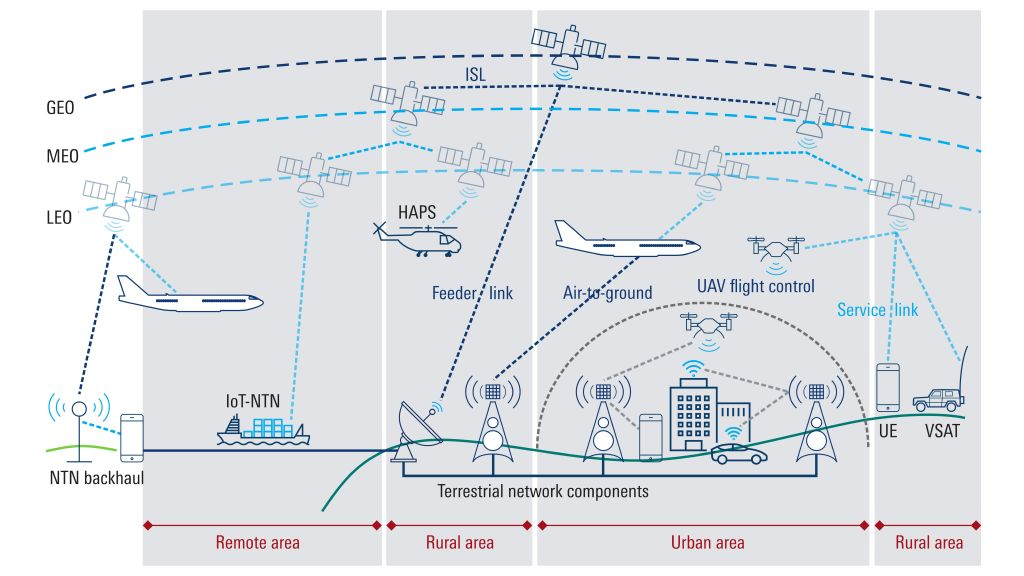
\includegraphics[width=0.9\textwidth]{res/multilayered-ntn.jpg}
    \caption{Complex multilayered \ac{NTN} scenario \cite{connecting-ntn-rohde-schwarz}}
    \label{fig:multilayered-ntn}
\end{figure}

In \cite{potential-multilayered-nierarchical-ntn-wang} it has been shown that the use of \ac{HAP} as relays between the ground segment of the network and the upper \ac{GEO} satellite links can deliver up to six times the capacity, and better overall outage probability, than point-to-point \ac{GEO} transmissions.


\section{Types of payloads}
When implementing a non-terrestrial network, an important choice to be made is the type of payload to use. Each one of the two main presented categories has its own benefits as briefly described below.

\subsection{Bent-pipe payload}
\label{sec:bent-pipe-payload}
This is the simplest approach, where the role of the satellite consists only of  repeating the signal received from the \ac{UE} on the ground towards the terrestrial gateway. Configurations such as the one depicted in Fig. \ref{fig:ntn-bent-pipe} go by the name of bent pipe payloads and are characterized by the presence of a terrestrial g-NodeB, while the satellite has the sole purpose of providing a transparent link with the \ac{UE}.

While such solutions are by far the simplest in terms of payload complexity, the main drawback is the even longer experienced latency, since communications between users served by the same satellite would also have to be routed through the terrestrial gateway, increasing the latency by at least two times the propagation delay.
This scenario also poses strict bandwidth requirements on the feeder link, since all the traffic must necessarily pass through it.
Other, smarter, solutions are able to route at least part of the inbound traffic autonomously, without routing everything back to earth.

\begin{figure}[ht]
    \centering
    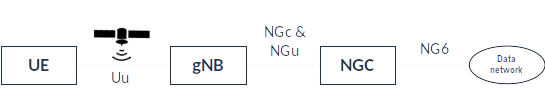
\includegraphics[width=0.9\textwidth]{res/ntn-bent-pipe.png}
    \caption{NTN with access network based on satellites with bent pipe payload \cite{3gpp-tr-38.811}}
    \label{fig:ntn-bent-pipe}
\end{figure}

\subsection{On-board g-NodeB}
\label{sec:onboard-gnb}
A slightly more sophisticated approach foresees the installation of g-NodeB capabilities directly onto the satellite payload. This has the benefit of reducing the experienced latency in some cases, as well as reducing the utilization of the feeder link. Certain protocols, designed to terminate at the \ac{gNB}, can in this case reach their designated endpoint without necessitating to be routed back to the ground gateway.

Figure \ref{fig:ntn-gnb-onboard} from \cite{3gpp-tr-38.811} shows the architecture of a \ac{NTN} using access network based on satellites with \ac{gNB} on board as payload.

\begin{figure}[ht]
    \centering
    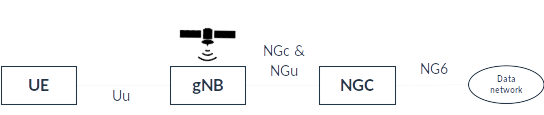
\includegraphics[width=0.9\textwidth]{res/ntn-regen.png}
    \caption{NTN with access network based on satellites with on-board gNB payload \cite{3gpp-tr-38.811}}
    \label{fig:ntn-gnb-onboard}
\end{figure}

\section{Available commercial solutions}
\paragraph{Legacy solutions}
Commercial solutions, first concerning satellite-based phone calls and successively evolved to provide internet access, have been available since a long time. However, the majority of this legacy infrastructure makes use of \ac{GEO} satellites, therefore presenting all the limitations discussed in section \ref{sec:satellite-types}, offering limited throughput and large delays. Such constraints render this technology not suitable for the needs of modern internet connections standards.

\paragraph{Recent developments}
While commercial solutions using \ac{LEO} satellites are starting to appear, enjoying some degree of success with notable examples such as the one presented in section \ref{sec:leo}, all of those solutions make use of many proprietary protocols to allow for the communication to take place, and up until now no internationally agreed standard has been defined.

This is where most of the research is currently being conducted and where the business world is posing its attention due to the characteristics of \ac{LEO} satellites that makes them the most suited to provide high speed satellite internet access.